\section{LOWER-LEVEL PROCESSES\label{app:lower_level_processes}}

\begin{figure}[h]
	\centering
	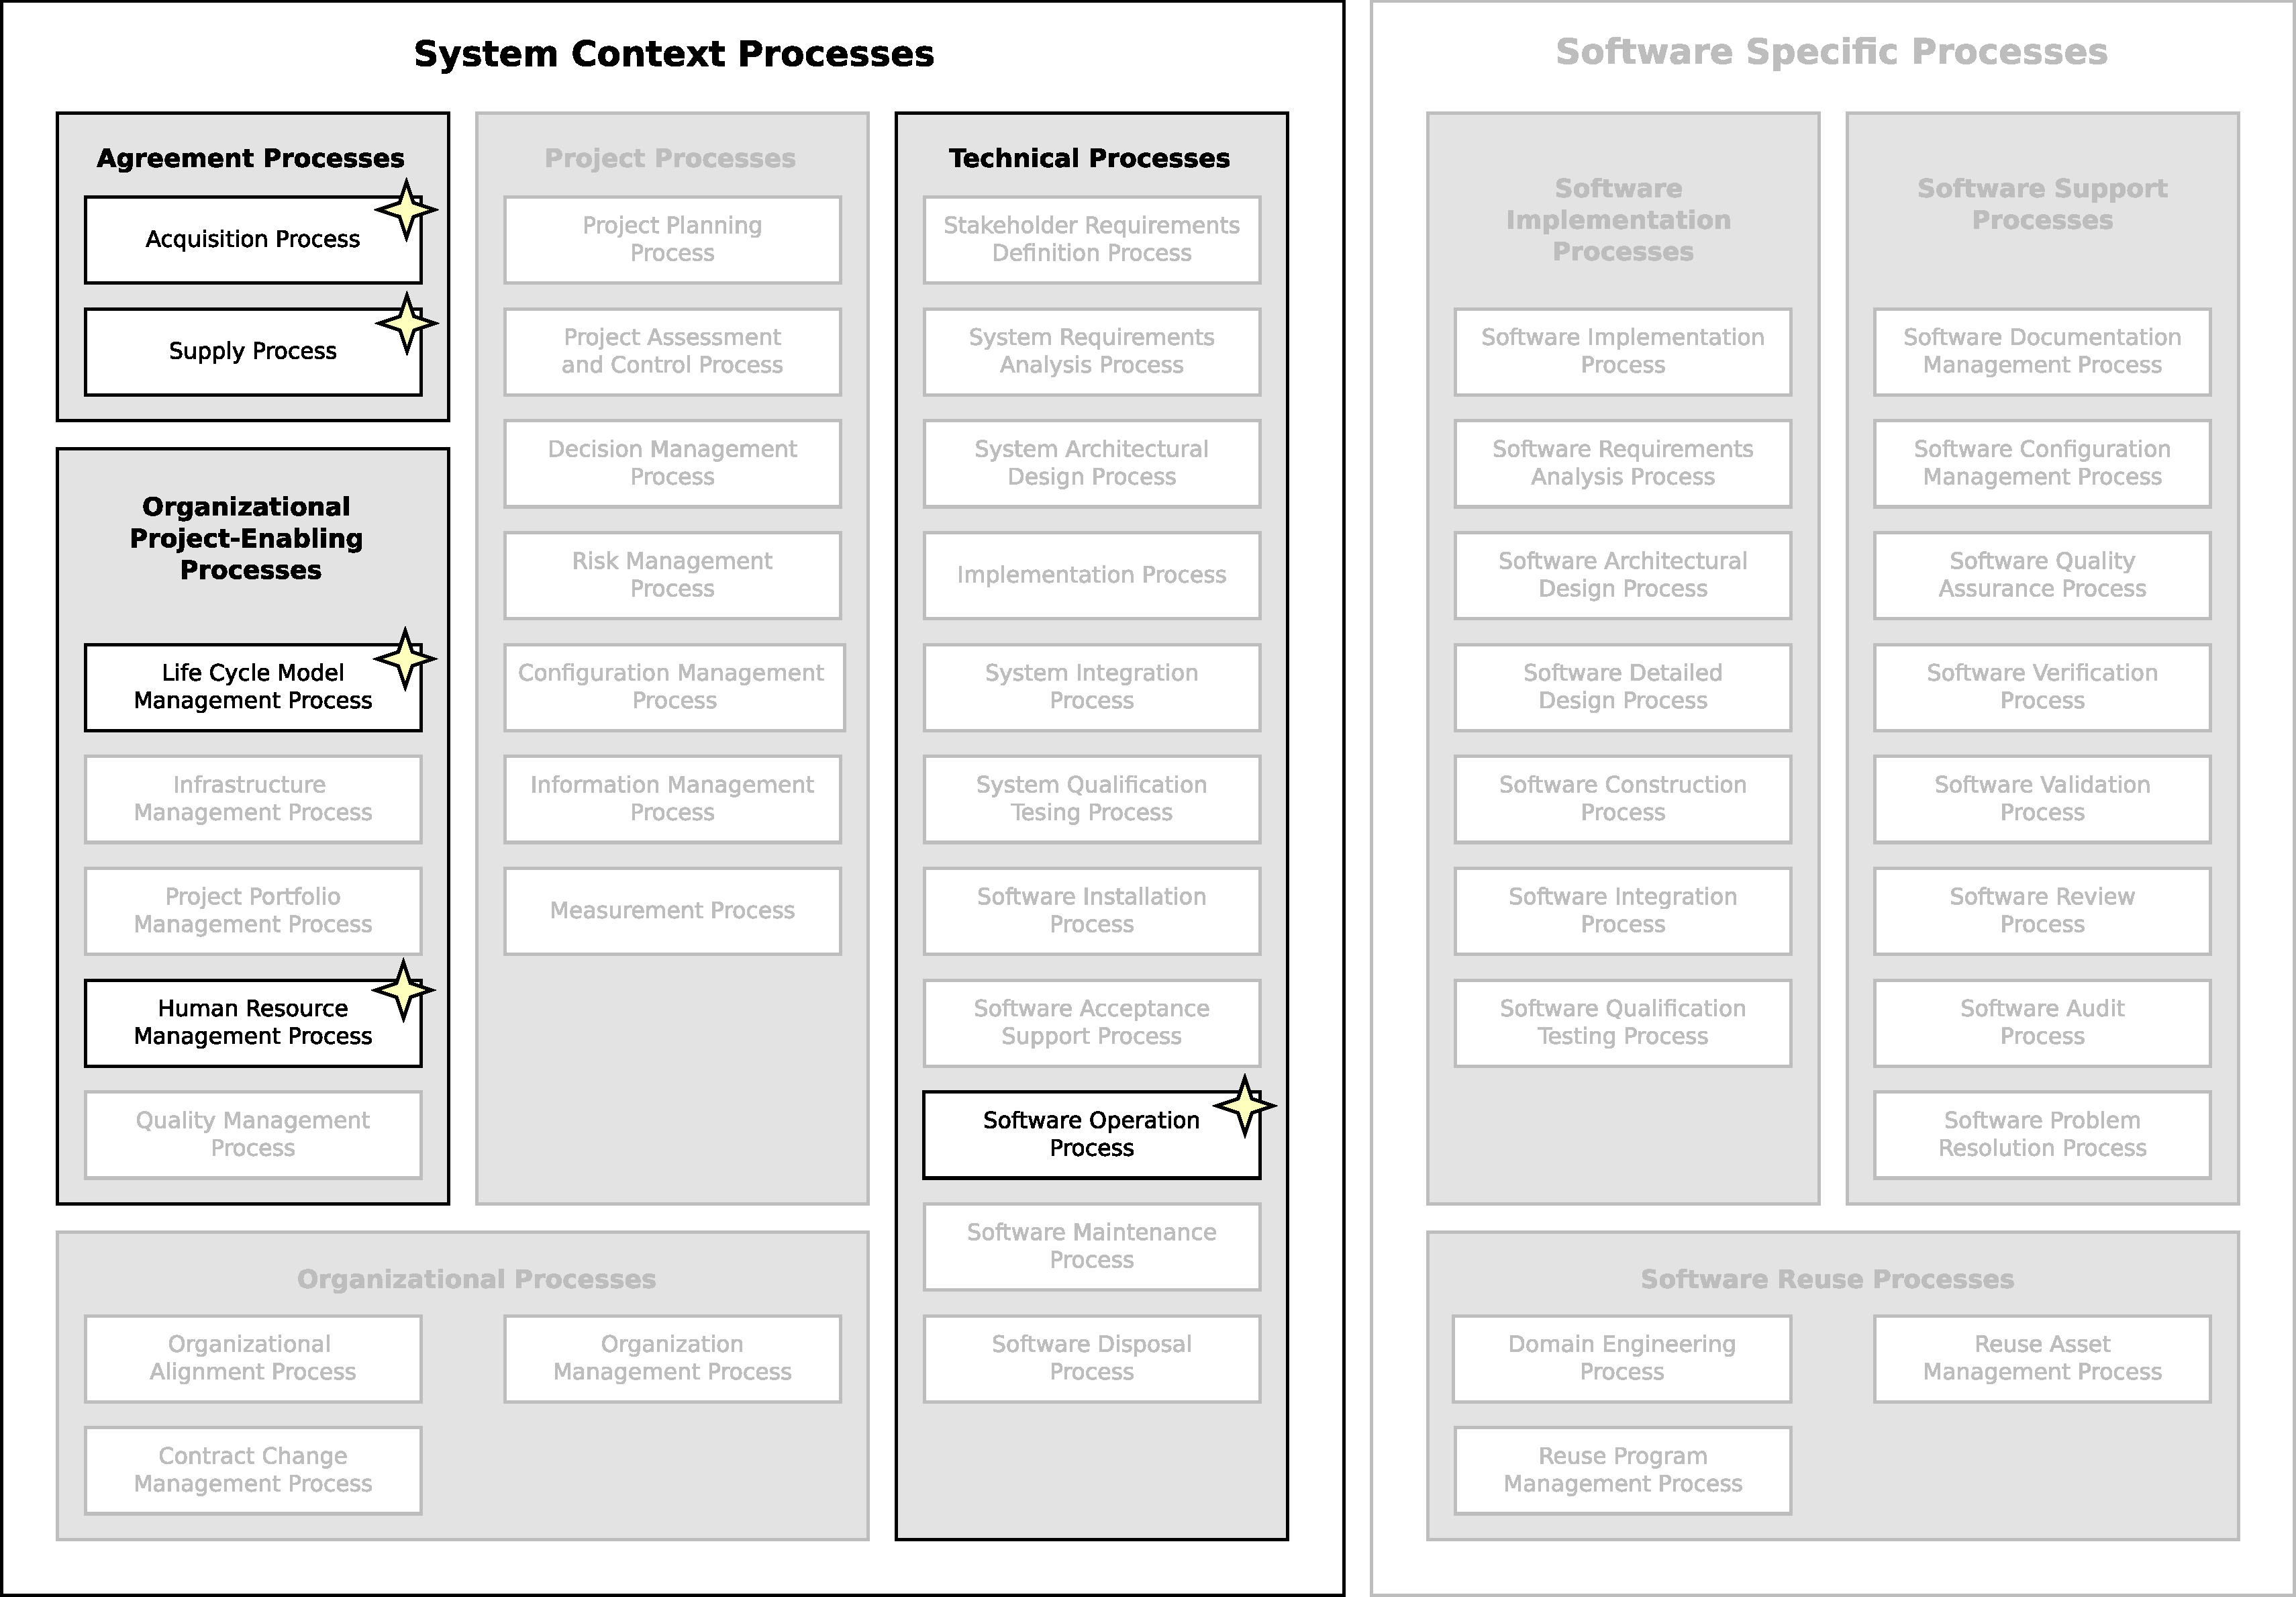
\includegraphics[width=15cm,keepaspectratio]{figures/life-cycle-process-groups-lower-level-processes.pdf}
	\caption{PROCESS REFERENCE MODEL (PRM) LOWER-LEVEL PROCESSES}
	\label{fig:lower_level_processes}
\end{figure}

\begin{adjustwidth}{1em}{0pt}

	Some of the processes defined within this standard may require additional lower-level processes in order to be realized in certain industries or by certain businesses whose activities are directed or more specific than the processes defined in the primary content of the document seemingly allow.

	Only the purpose and outcomes for these processes has been defined, and the necessary activities for the processes, as they relate to those found in the parent-level process, need to be integrated into said process' activities and tasks in order to extend, and not disrupt, the parent-level process' outcomes, activities, and tasks. 

\end{adjustwidth}

	\newpage
	\subsection{ACQUISITION PROCESS LOWER-LEVEL PROCESSES\label{llsubsec:acquisition_processes}}
	\begin{figure}[h]
		\centering
		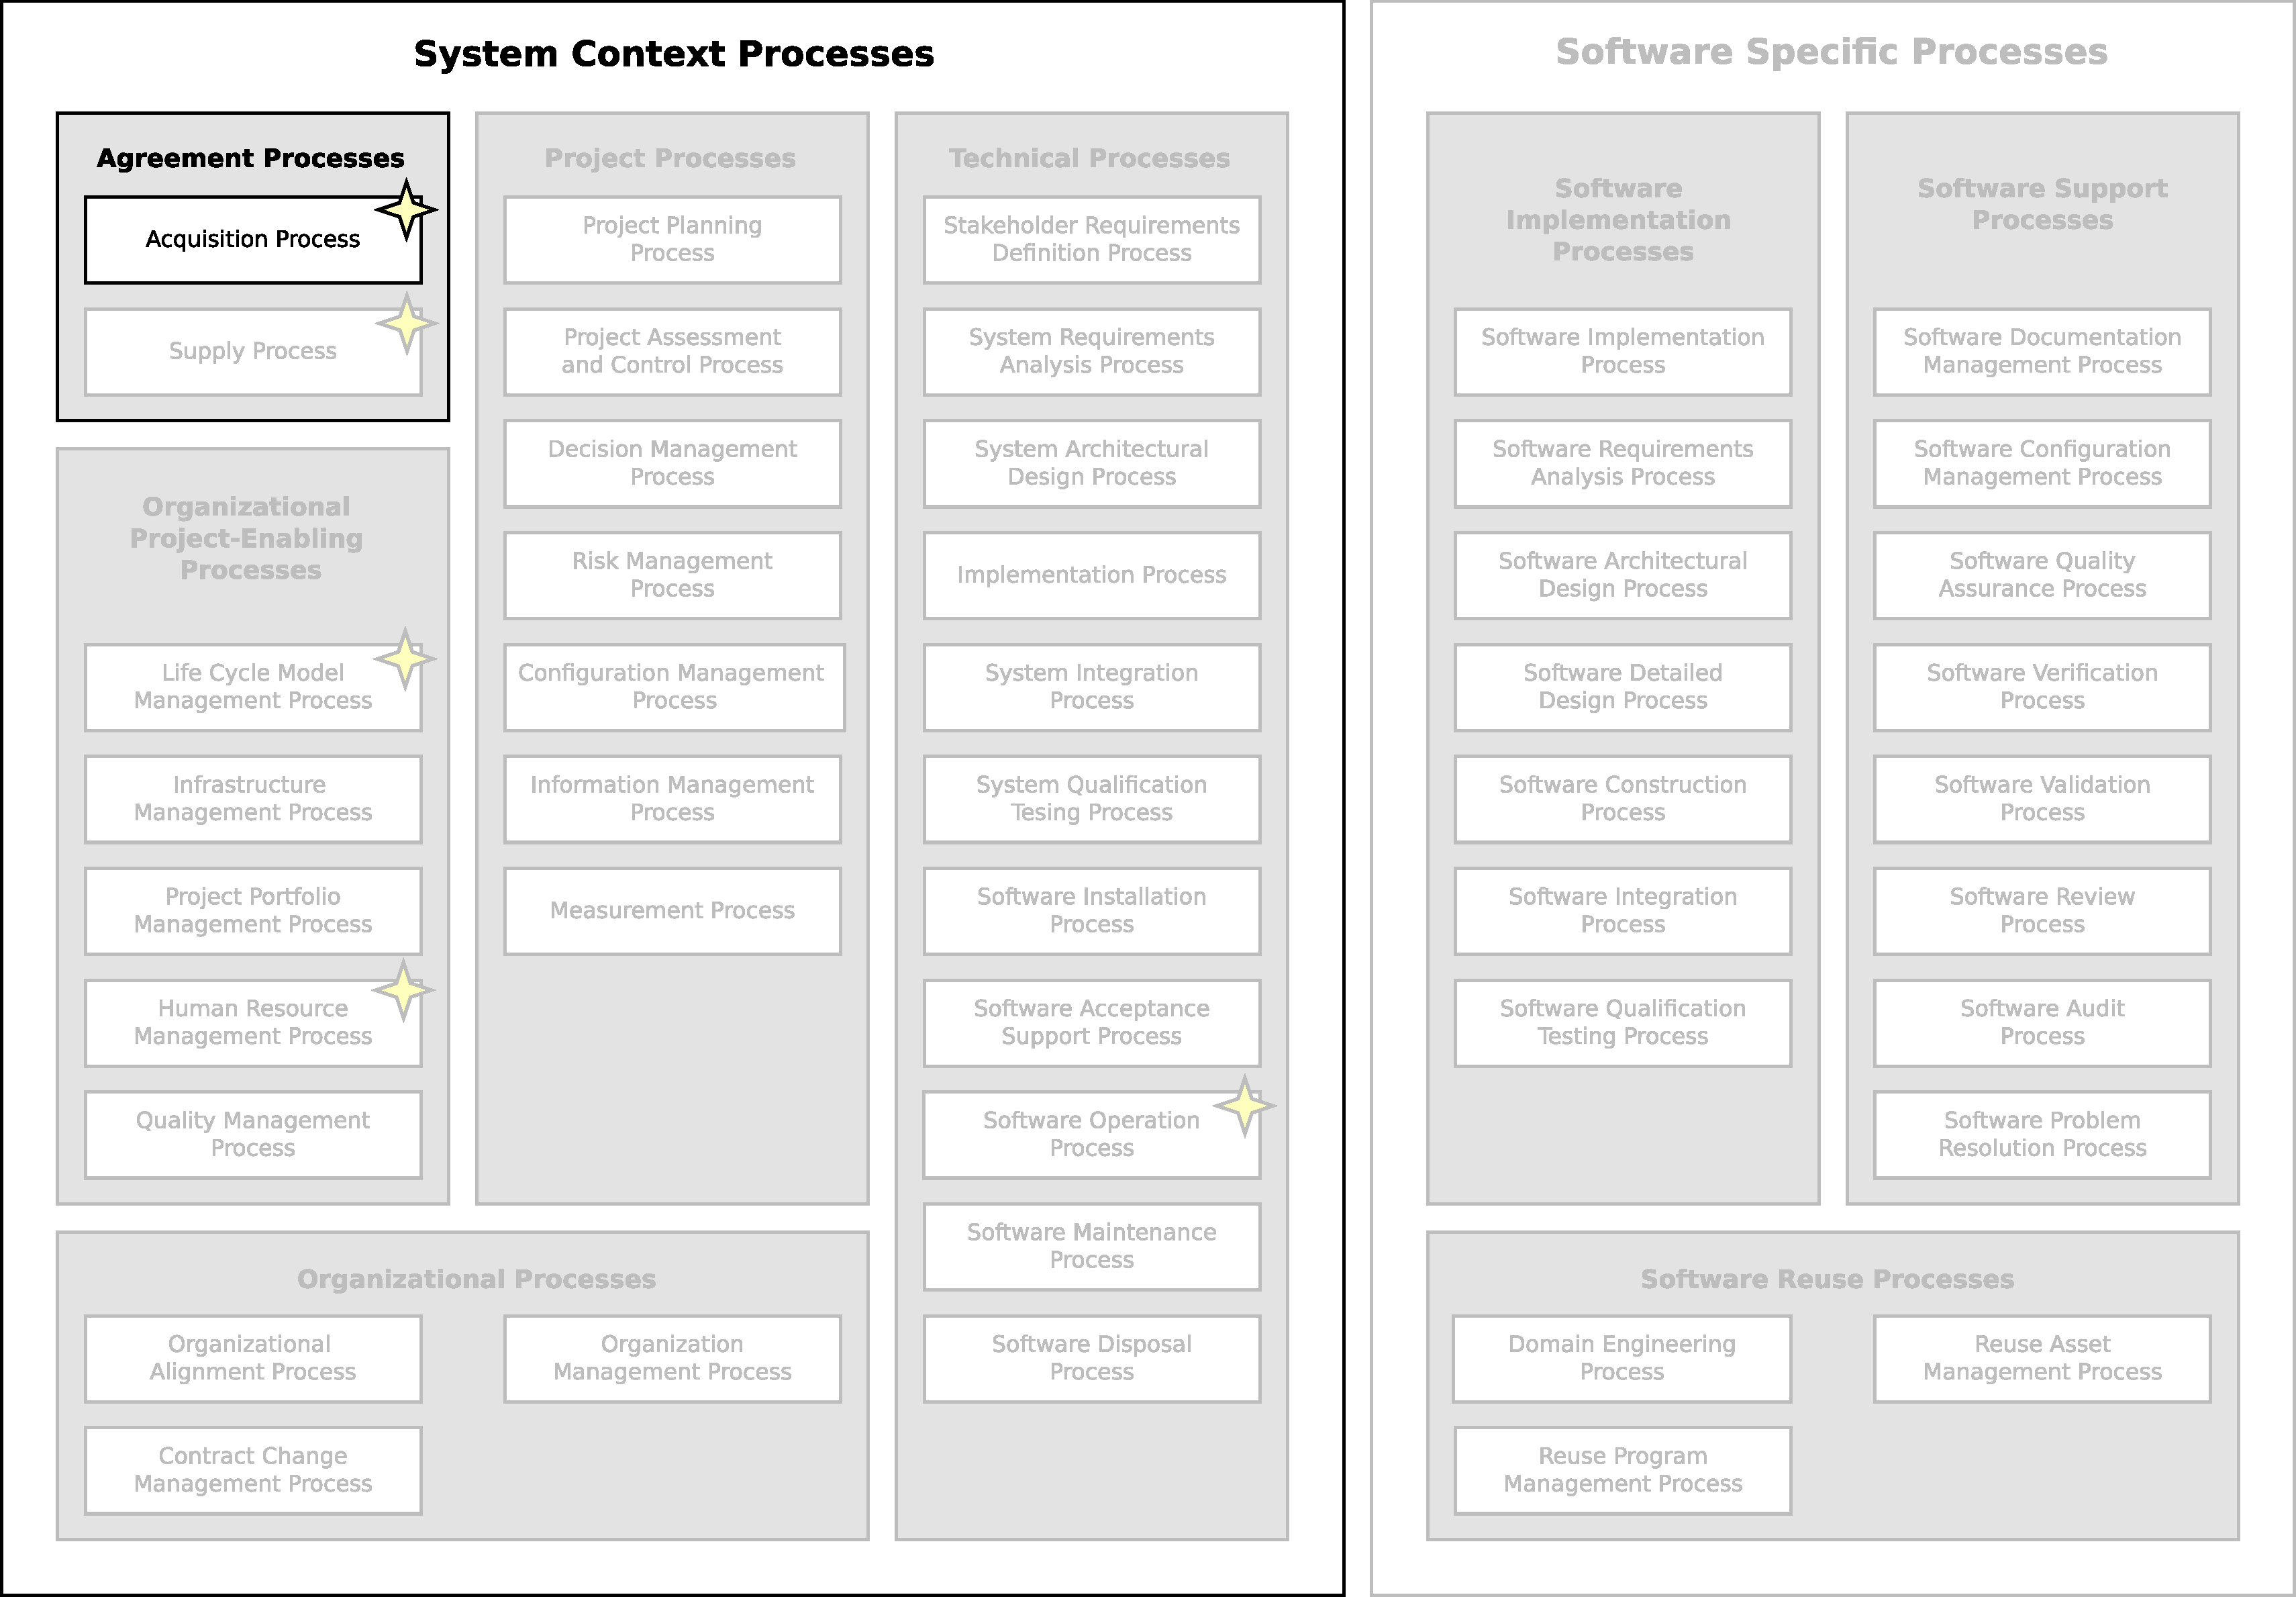
\includegraphics[width=15cm,keepaspectratio]{figures/life-cycle-process-groups-lower-level-acquisition-processes.pdf}
		\caption{Acquisition Process Lower-Level Processes}
		\label{fig:lower_level_acquisition_processes}
	\end{figure}

		\subsubsection{ACQUISITION PREPARATION PROCESS\label{llproc:acquisition_preparation_process}}

			\subsubsubsection{PURPOSE}
			\begin{adjustwidth}{2em}{0pt} 

				The purpose of the \nameref{llproc:acquisition_preparation_process} is to establish the needs and goals of the acquisition and to communicate these with the potential suppliers.

				This process is a lower-level process of the \nameref{proc:acquisition_process}, that replaces the Acquisition Preparation activity.

			\end{adjustwidth}

			\subsubsubsection{OUTCOMES}
			\begin{adjustwidth}{2em}{0pt} 

				\begin{compactitem}

					\item the concept or the need for the acquisition, development, or enhancement is established;

					\item stakeholder requirements are defined;

					\item an acquisition strategy is developed; and

					\item supplier selection criteria are defined.

				\end{compactitem}

			\end{adjustwidth}

		\subsubsection{SUPPLIER SELECTION PROCESS\label{llproc:supplier_selection_process}}

			\subsubsubsection{PURPOSE}
			\begin{adjustwidth}{2em}{0pt} 

				The purpose of the \nameref{llproc:supplier_selection_process} is to choose the organization that is to be responsible for the delivery of the requirements of the project.

				This process is a lower-level process of the \nameref{proc:acquisition_process}, that replaces the Supplier Selection activity.

			\end{adjustwidth}

			\subsubsubsection{OUTCOMES}
			\begin{adjustwidth}{2em}{0pt} 

				\begin{compactitem}

					\item the supplier selection criteria are established and used to evaluate potential suppliers;

					\item the supplier is selected based upon the evaluation of the supplier's proposals, process capabilities, and other factors; and

					\item an agreement is established and negotiated between the acquirer and the supplier.

				\end{compactitem}

			\end{adjustwidth}

		\subsubsection{AGREEMENT MONITORING PROCESS\label{llproc:agreement_monitoring_process}}

			\subsubsubsection{PURPOSE}
			\begin{adjustwidth}{2em}{0pt} 

				The purpose of the \nameref{llproc:agreement_monitoring_process} is to track and assess performance of the supplier against agreed requirements.

				This process is a lower level-process of the \nameref{proc:acquisition_process}. It replaces the Agreement Monitoring activity.

			\end{adjustwidth}

			\subsubsubsection{OUTCOMES}
			\begin{adjustwidth}{2em}{0pt} 

				\begin{compactitem}

					\item joint activities between the acquirer and the supplier are performed as needed;

					\item information on technical progress is exchanged regularly with the supplier;

					\item performance of the supplier is monitored against the agreed requirements; and

					\item agreement changes, if needed, are negotiated between the acquirer and the supplier and documented in the agreement.

				\end{compactitem}

			\end{adjustwidth}

		\subsubsection{ACQUIRER ACCEPTANCE PROCESS\label{llproc:acquirer_acceptance_process}}

			\subsubsubsection{PURPOSE}
			\begin{adjustwidth}{2em}{0pt} 

				The purpose of the \nameref{llproc:acquirer_acceptance_process} is to approve the supplier's deliverable when all acceptance criteria are satisfied.

				This process is a lower-level process of the \nameref{proc:acquisition_process}. It replaces the Acquirer Acceptance activity.

			\end{adjustwidth}

			\subsubsubsection{OUTCOMES}
			\begin{adjustwidth}{2em}{0pt} 

				\begin{compactitem}

					\item the delivered software product and/or service are evaluated with regard to the agreement;

					\item the acquirer's acceptance is based on the agreed acceptance criteria; and

					\item the software product and/or service is accepted by the acquirer.

				\end{compactitem}

			\end{adjustwidth}



	\newpage
	\subsection{SUPPLY PROCESS LOWER-LEVEL PROCESSES\label{llsubsec:supply_processes}}
	\begin{figure}[h]
		\centering
		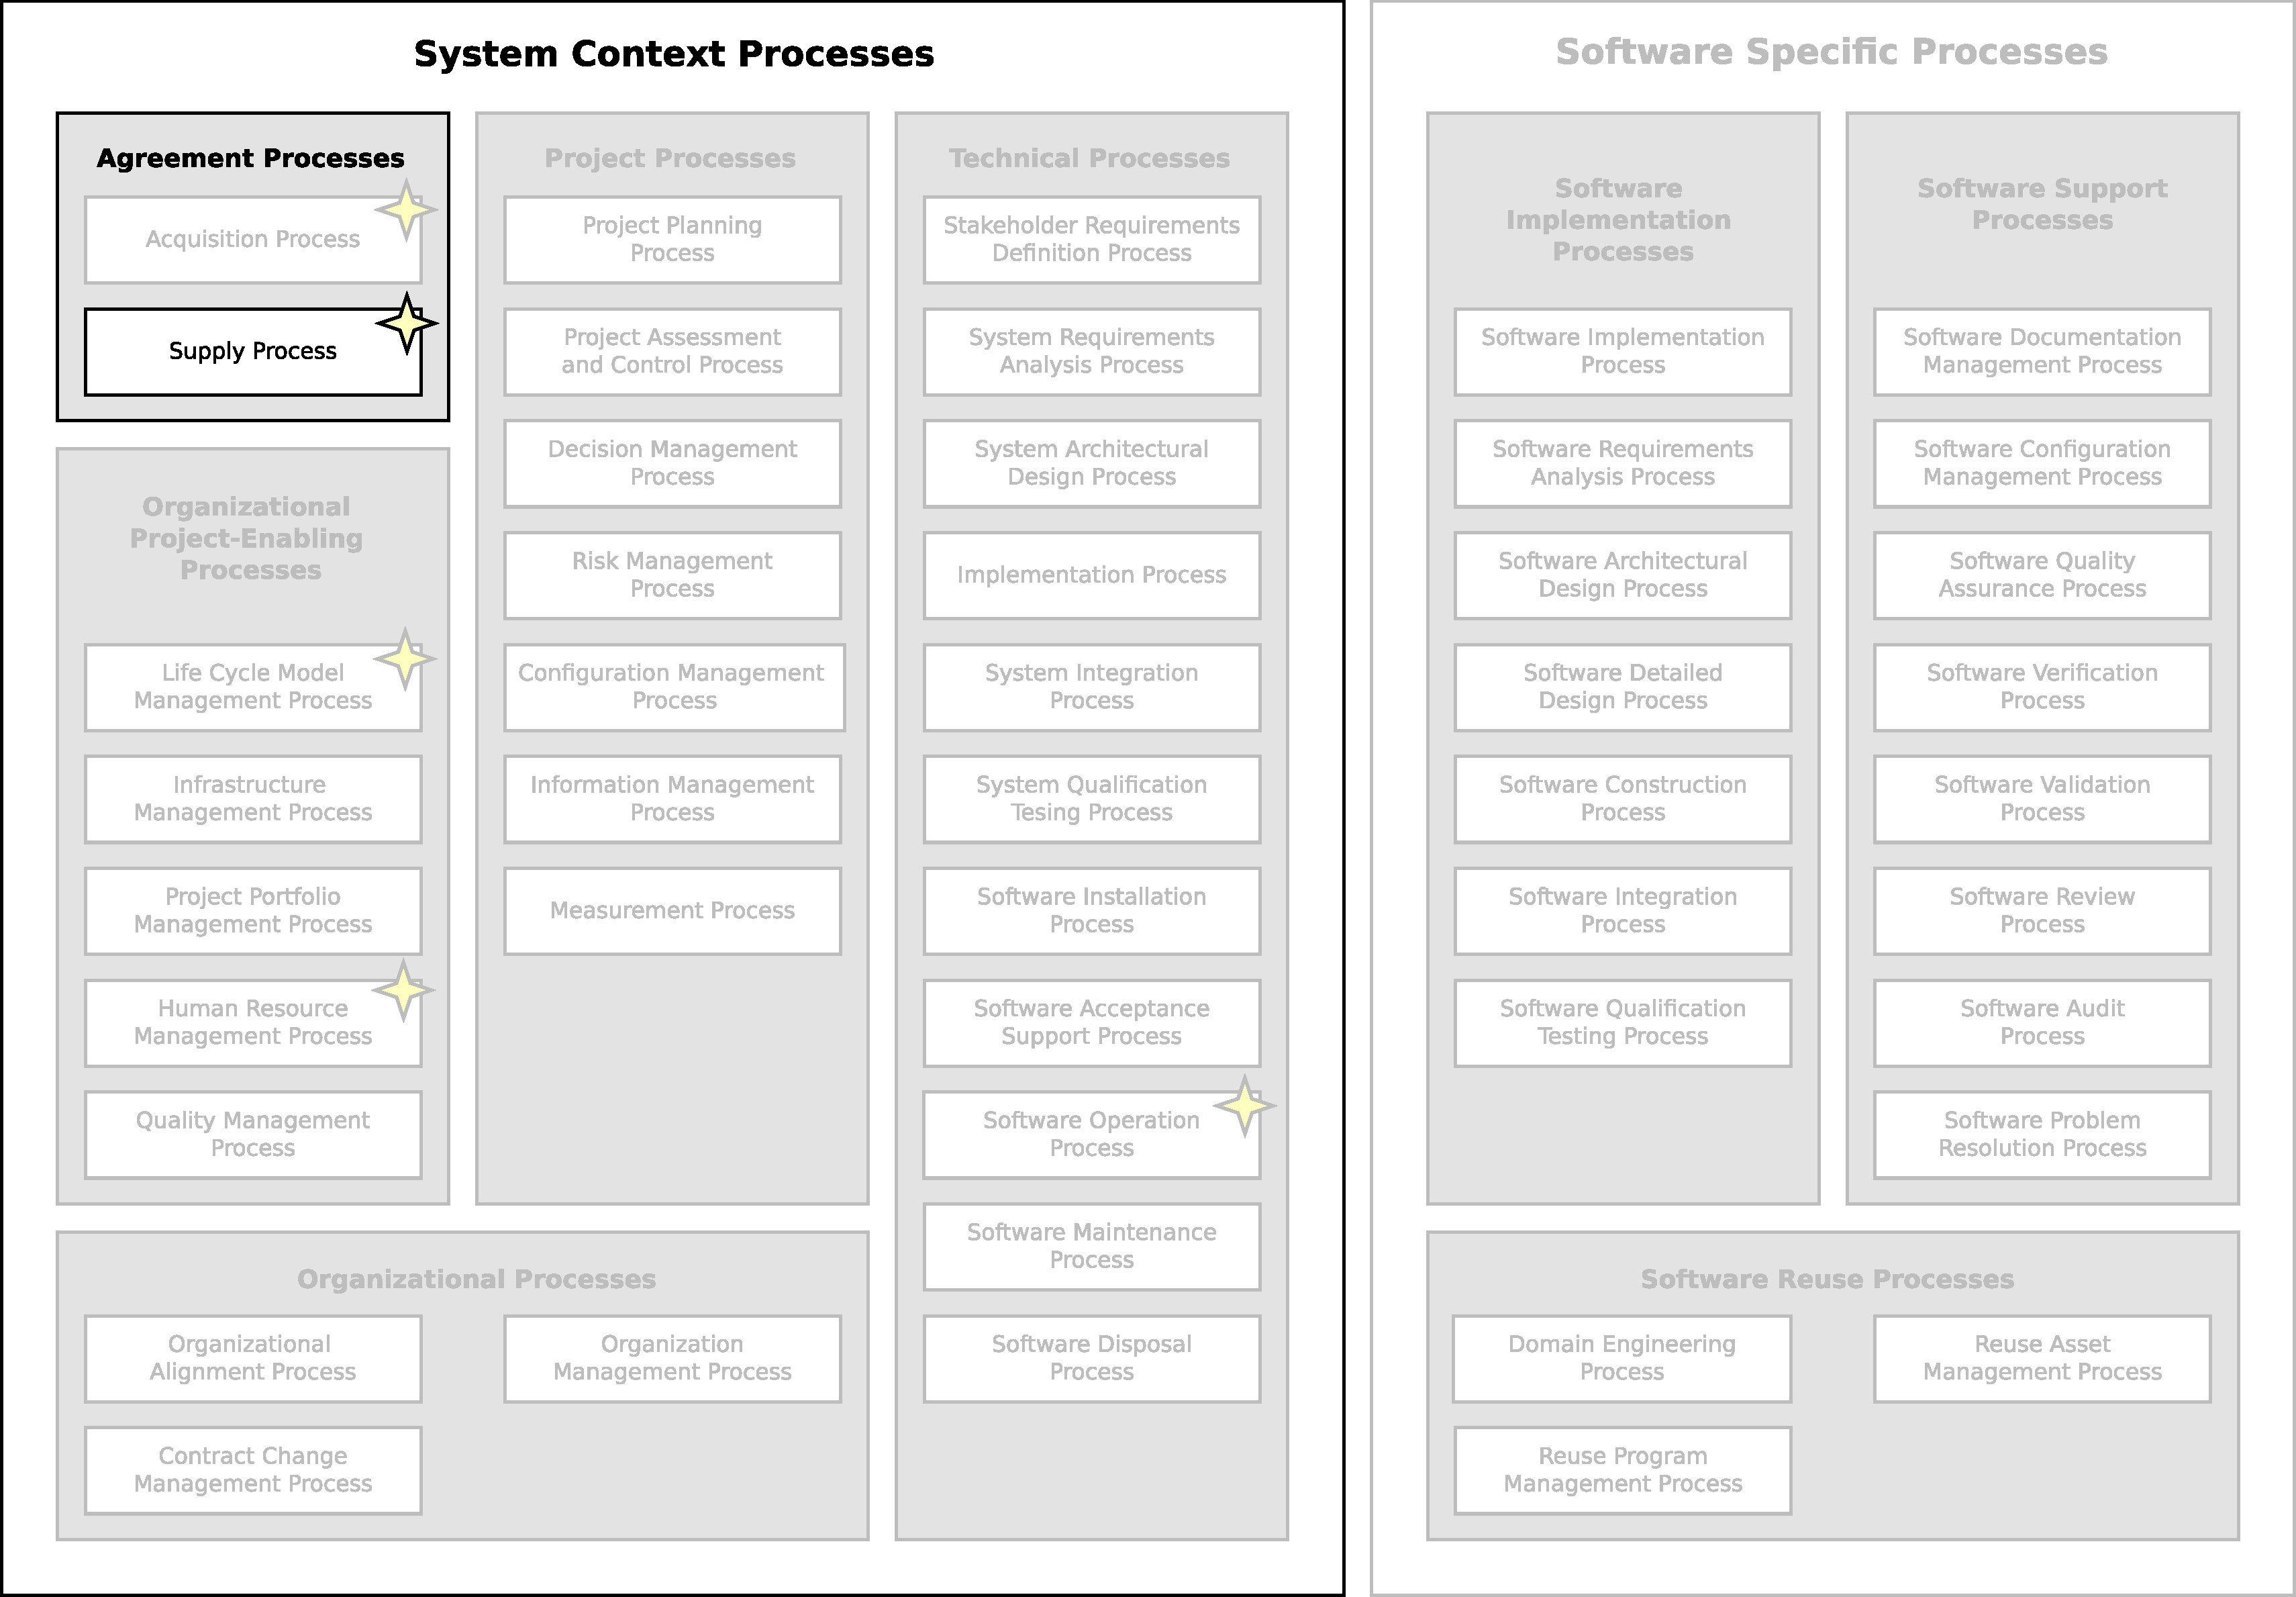
\includegraphics[width=15cm,keepaspectratio]{figures/life-cycle-process-groups-lower-level-supply-processes.pdf}
		\caption{Supply Process Lower-Level Processes}
		\label{fig:lower_level_supply_processes}
	\end{figure}
		
		\subsubsection{SUPPLIER TENDERING PROCESS\label{llproc:supplier_tendering_process}}

			\subsubsubsection{PURPOSE}
			\begin{adjustwidth}{2em}{0pt} 

				The purpose of the \nameref{llproc:supplier_tendering_process} is to establish an interface to respond to acquirer inquiries and requests for proposal, prepare and submit proposals.

				This process is a lower level-process of the \nameref{proc:supply_process}. It replaces the Supplier Tendering activity.

			\end{adjustwidth}

			\subsubsubsection{OUTCOMES}
			\begin{adjustwidth}{2em}{0pt} 

				\begin{compactitem}

					\item a communication interface is established and maintained in order to respond to acquirer inquiries and requests for proposal;

					\item requests for proposal are evaluated according to defined criteria to determine whether or not to submit a proposal;

					\item the need to undertake preliminary surveys or feasibility studies is determined;

					\item suitable resources are identified to perform the proposed work; and

					\item a supplier proposal is prepared and submitted in response to the acquirer request.

				\end{compactitem}

			\end{adjustwidth}

		\subsubsection{CONTRACT AGREEMENT PROCESS\label{llproc:contract_agreement_process}}

			\subsubsubsection{PURPOSE}
			\begin{adjustwidth}{2em}{0pt} 
				
				The purpose of \nameref{llproc:contract_agreement_process} is to negotiate and approve a contract/agreement that clearly and unambiguously specifies the expectations, responsibilities, work products/deliverables and liabilities of both the supplier and the acquirer.

				This process is a lower level-process of the \nameref{proc:supply_process}. It replaces the Contract Agreement activity.

			\end{adjustwidth}

			\subsubsubsection{OUTCOMES}
			\begin{adjustwidth}{2em}{0pt} 

				\begin{compactitem}

					\item a contract/agreement is negotiated, reviewed, approved and awarded to the supplier(s);

					\item mechanisms for monitoring the capability and performance of the supplier(s) and for mitigation of identified risks are reviewed and considered for inclusion in the contract conditions;

					\item proposers/tenderers are notified of the result of proposal/tender selection; and

					\item formal confirmation of agreement is obtained.

				\end{compactitem}

			{\bf Note}: The \nameref{llproc:contract_agreement_process} is used to obtain formal confirmation of assignments that were offered during the \nameref{llproc:supplier_tendering_process}.


			\end{adjustwidth}

		\subsubsection{PRODUCT AND SERVICE DELIVERY AND SUPPORT PROCESS\label{llproc:product_and_service_delivery_and_support_process}}

			\subsubsubsection{PURPOSE}
			\begin{adjustwidth}{2em}{0pt} 

				The purpose of the \nameref{llproc:product_and_service_delivery_and_support_process} is to provide the specified product or service to the acquirer with support appropriate to achieve confidence that the requirements have been met.

				This process is a lower-level process of the \nameref{proc:supply_process}. It replaces the Product/Service Delivery and Support activity.

			\end{adjustwidth}

			\subsubsubsection{OUTCOMES}
			\begin{adjustwidth}{2em}{0pt} 

				\begin{compactitem}

					\item the contents of the product release are determined;

					\item the release is assembled from configured items;

					\item the release documentation is defined and produced;

					\item the release delivery mechanism and media are determined;

					\item release approval is effected against defined criteria;

					\item the product release is made available to the acquirer;

					\item confirmation of release is obtained;

					\item the product is completed and delivered to the acquirer;

					\item acquirer acceptance tests and reviews are supported;

					\item the product is put into operation in the customers’ environment; and

					\item problems detected during acceptance are identified and communicated to those responsible for resolution.

				\end{compactitem}

			{\bf Note}: Incremental delivery would be in completed increments.

			\end{adjustwidth}


	\newpage
	\subsection{LIFE CYCLE MODEL MANAGEMENT PROCESS LOWER-LEVEL PROCESSES\label{llsubsec:life_cycle_model_management_processes}}
	\begin{figure}[h]
		\centering
		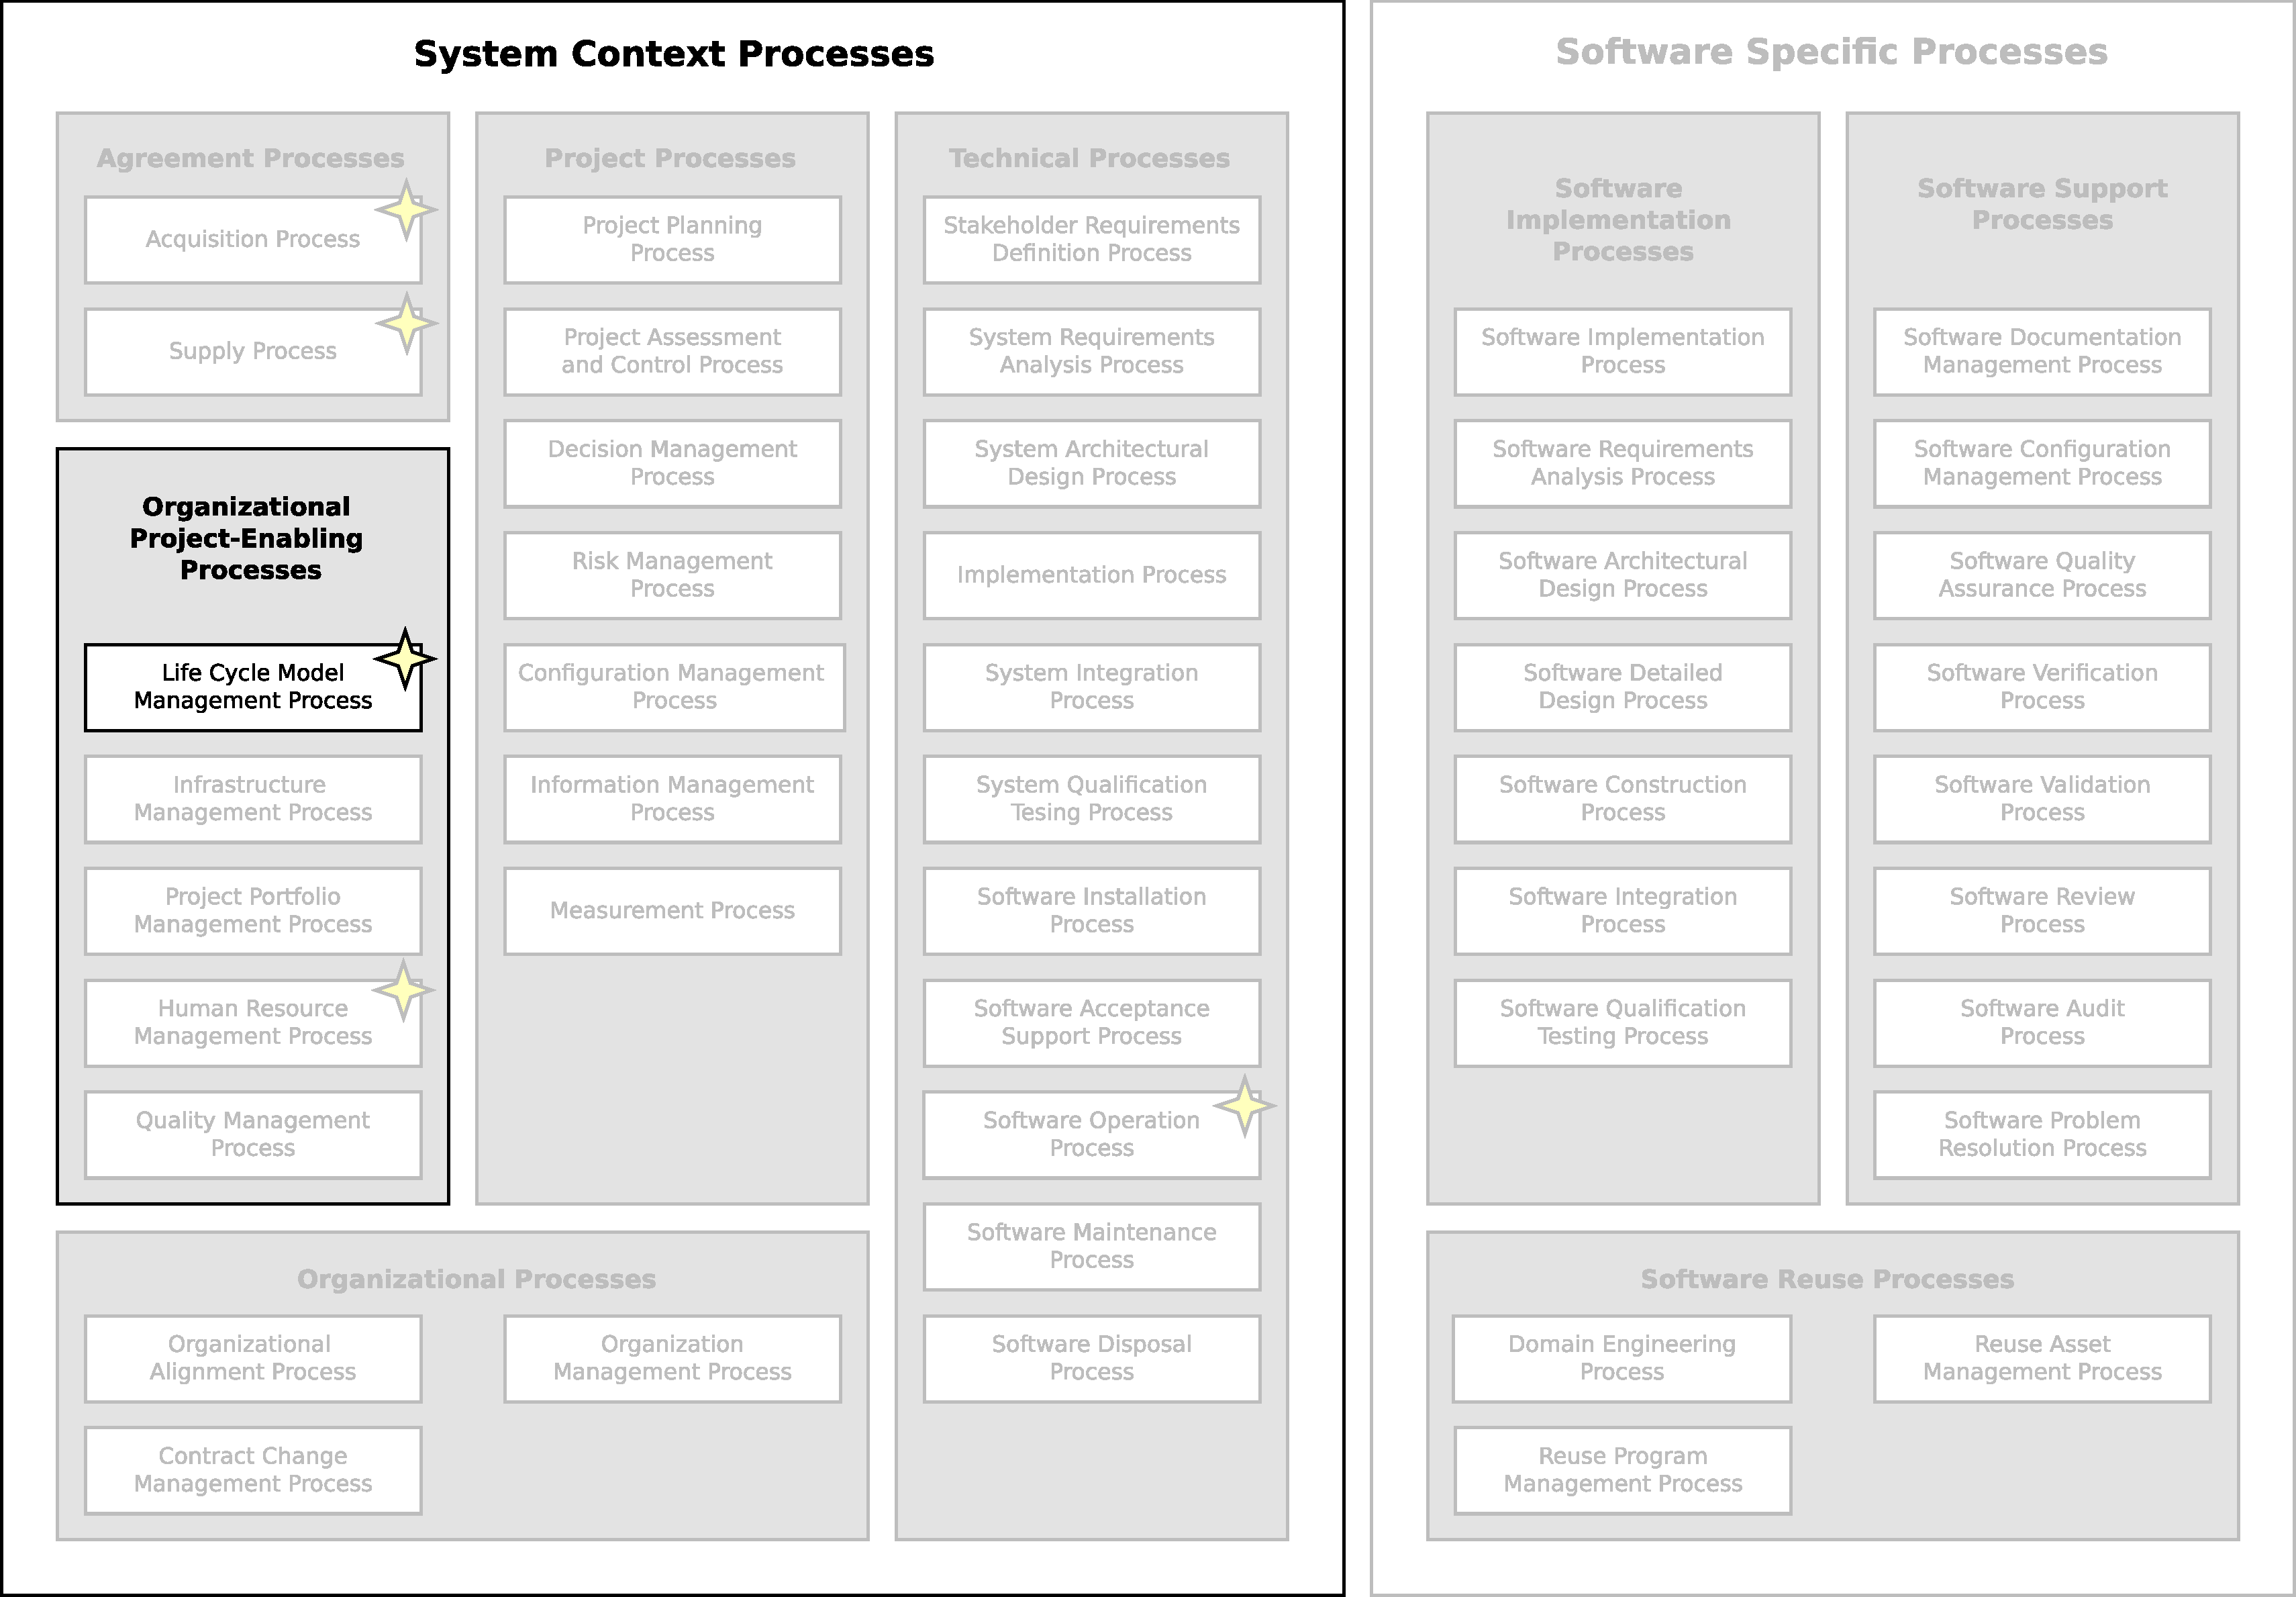
\includegraphics[width=15cm,keepaspectratio]{figures/life-cycle-process-groups-lower-level-life-cycle-model-management-processes.pdf}
		\caption{Life Cycle Model Management Process Lower-Level Processes}
		\label{fig:lower_level_life_cycle_model_management_processes}
	\end{figure}

		\subsubsection{PROCESS ESTABLISHMENT PROCESS\label{llproc:process_establishment_process}}

			\subsubsubsection{PURPOSE}
			\begin{adjustwidth}{2em}{0pt} 

				The purpose of the \nameref{llproc:process_establishment_process} is to establish a suite of organizational processes for all life cycle processes as they apply to its business activities.

				This process is a lower-level process of the \nameref{proc:life_cycle_model_management_process}. It replaces the Process Establishment activity.

			\end{adjustwidth}

			\subsubsubsection{OUTCOMES}
			\begin{adjustwidth}{2em}{0pt} 

				\begin{compactitem}

					\item a defined and maintained standard set of processes are established, along with an indication of each process's applicability;

					\item the detailed tasks, activities and associated work products of the standard process are identified, together with expected performance characteristics;

					\item a strategy for tailoring the standard process for the product or service is developed in accordance with the needs of the project; and

					\item information and data related to the use of the standard process for specific projects exist and are maintained.

				\end{compactitem}

			\end{adjustwidth}

		\subsubsection{PROCESS ASSESSMENT PROCESS\label{llproc:process_assessment_process}}

			\subsubsubsection{PURPOSE}
			\begin{adjustwidth}{2em}{0pt} 
				
				The purpose of the \nameref{llproc:process_assessment_process} is to determine the extent to which the organization's standard processes contribute to the achievement of its business goals and to help the organization focus on the need for continuous process improvement.

				This process is a lower-level process of the \nameref{proc:life_cycle_model_management_process}, that replaces its Process Assessment activity.

			\end{adjustwidth}

			\subsubsubsection{OUTCOMES}
			\begin{adjustwidth}{2em}{0pt} 

				\begin{compactitem}

					\item information and data related to the use of the standard process for specific projects exists and is maintained;

					\item the relative strengths and weaknesses of the organization's standard processes are understood; and

					\item accurate and accessible assessment records are kept and maintained.

				\end{compactitem}

			\end{adjustwidth}

		\subsubsection{PROCESS IMPROVEMENT PROCESS\label{llproc:process_improvement_process}}

			\subsubsubsection{PURPOSE}
			\begin{adjustwidth}{2em}{0pt} 
				
				The purpose of the \nameref{llproc:process_improvement_process} is to continually improve the organization's effectiveness and efficiency through the processes used and maintained and aligned with the business need.

				This process is a lower-level process of the \nameref{proc:life_cycle_model_management_process}, that replaces its Process Improvement activity.

			\end{adjustwidth}

			\subsubsubsection{OUTCOMES}
			\begin{adjustwidth}{2em}{0pt} 

				\begin{compactitem}

					\item commitment is established to provide resources to sustain improvement actions;

					\item issues arising from the organization's internal/external environment are identified as improvement opportunities and justified as reasons for change;

					\item analysis of the current status of the existing process is performed, focusing on those processes from which improvement stimuli arise;
					
					\item improvement goals are identified and prioritized, and consequent changes to the process are defined and implemented; 					

					\item the effects of process implementation are monitored and confirmed against the defined improvement goals;
					
					\item knowledge gained from the improvements is communicated within the organization; and

					\item the improvements made are evaluated and consideration given for using solutions elsewhere within the organization.

				\end{compactitem}


				{\bf Note 1}: Information sources providing input for change may include: process assessment results, audits, customer's satisfaction reports, organizational effectiveness/efficiency, cost of quality.

				{\bf Note 2}: The current status of processes may be determined by process assessment.


			\end{adjustwidth}


	\newpage
	\subsection{HUMAN RESOURCE MANAGEMENT PROCESS LOWER-LEVEL PROCESSES\label{llsubsec:human_resource_management_processes}}
	\begin{figure}[h]
		\centering
		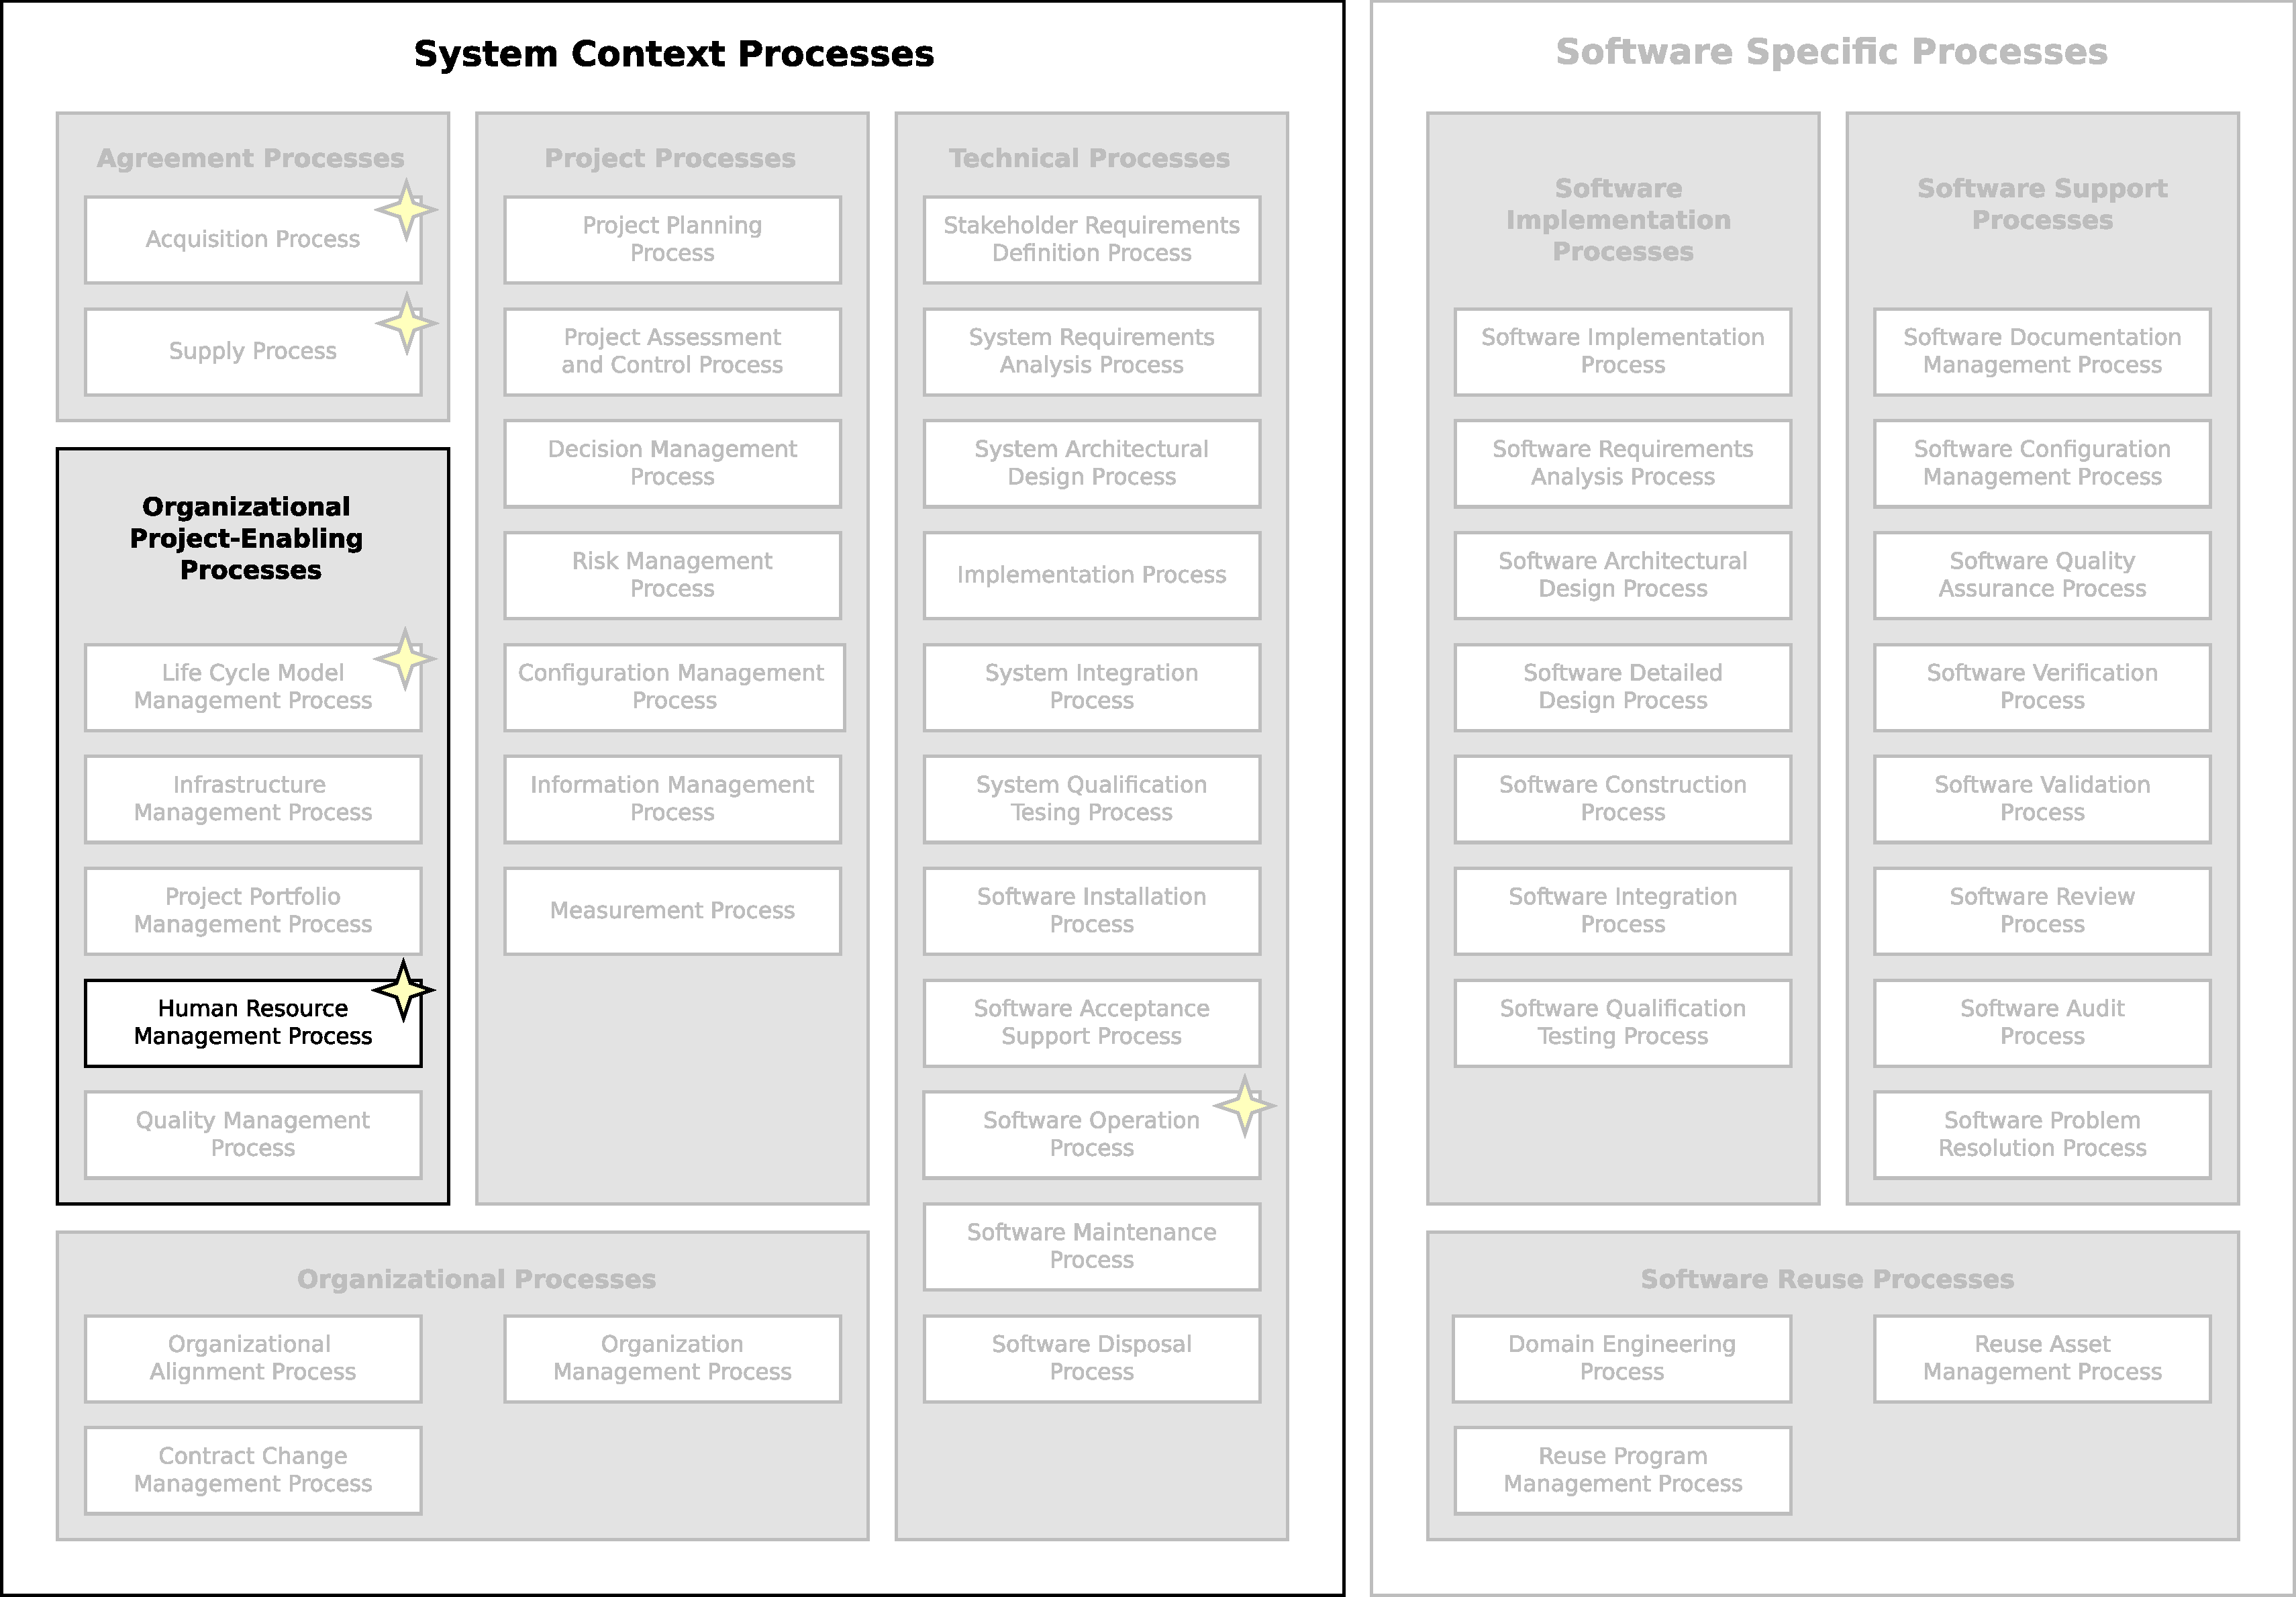
\includegraphics[width=15cm,keepaspectratio]{figures/life-cycle-process-groups-lower-level-human-resource-management-processes.pdf}
		\caption{Human Resource Management Lower-Level Processes}
		\label{fig:lower_level_human_resource_management_processes}
	\end{figure}

		\subsubsection{SKILL DEVELOPMENT PROCESS\label{llproc:skill_development_process}}

			\subsubsubsection{PURPOSE}
			\begin{adjustwidth}{2em}{0pt} 

				The purpose of the \nameref{llproc:skill_development_process} is to provide the organization and project with individuals who possess the needed skills and knowledge to perform their roles effectively.

				This process is a lower-level process of the \nameref{proc:human_resource_management_process}. It replaces the Skill Development activity.

			\end{adjustwidth}

			\subsubsubsection{OUTCOMES}
			\begin{adjustwidth}{2em}{0pt} 

				\begin{compactitem}

					\item training is developed or acquired to address the organization and project training needs; and

					\item training is conducted to ensure that all individuals have the skills required to perform their assignments, using mechanisms such as training strategies and materials.

				\end{compactitem}

			\end{adjustwidth}

		\subsubsection{SKILL ACQUISITION PROCESS\label{llproc:skill_acquisition_process}}

			\subsubsubsection{PURPOSE}
			\begin{adjustwidth}{2em}{0pt} 

				The purpose of the \nameref{llproc:skill_acquisition_process} is to provide the organization and projects with individuals who possess skills and knowledge to perform their roles effectively and to work together as a cohesive group.

				This process is a lower-level process of the \nameref{proc:human_resource_management_process}. It replaces the Skill Acquisition and Provision activity.

			\end{adjustwidth}

			\subsubsubsection{OUTCOMES}
			\begin{adjustwidth}{2em}{0pt} 

				\begin{compactitem}

					\item individuals with the required skills and competencies are identified and recruited;

					\item effective interaction between individuals and groups are supported;

					\item the work force have the skills to share information and co-ordinate their activities efficiently; and

					\item objective criteria are defined against which group and individual performance is monitored to provide performance feedback and to enhance performance.

				\end{compactitem}

			\end{adjustwidth}

		\subsubsection{KNOWLEDGE MANAGEMENT PROCESS\label{llproc:knowledge_management_process}}

			\subsubsubsection{PURPOSE}
			\begin{adjustwidth}{2em}{0pt} 

				The purpose of the \nameref{llproc:knowledge_management_process} is to ensure that individual knowledge, information and skills are collected, shared, reused and improved throughout the organization.

				This process is a lower-level process of the \nameref{proc:human_resource_management_process}. It replaces the Knowledge Management activity.

			\end{adjustwidth}

			\subsubsubsection{OUTCOMES}
			\begin{adjustwidth}{2em}{0pt} 

				\begin{compactitem}

					\item infrastructure is established and maintained for sharing common and domain information across the organization;

					\item knowledge is readily available and shared throughout the organization; and

					\item the organization selects an appropriate knowledge management strategy.

				\end{compactitem}

			\end{adjustwidth}


	\newpage
	\subsection{SOFTWARE OPERATION PROCESS LOWER-LEVEL PROCESSES\label{llsubsec:software_operation_processes}}
	\begin{figure}[h]
		\centering
		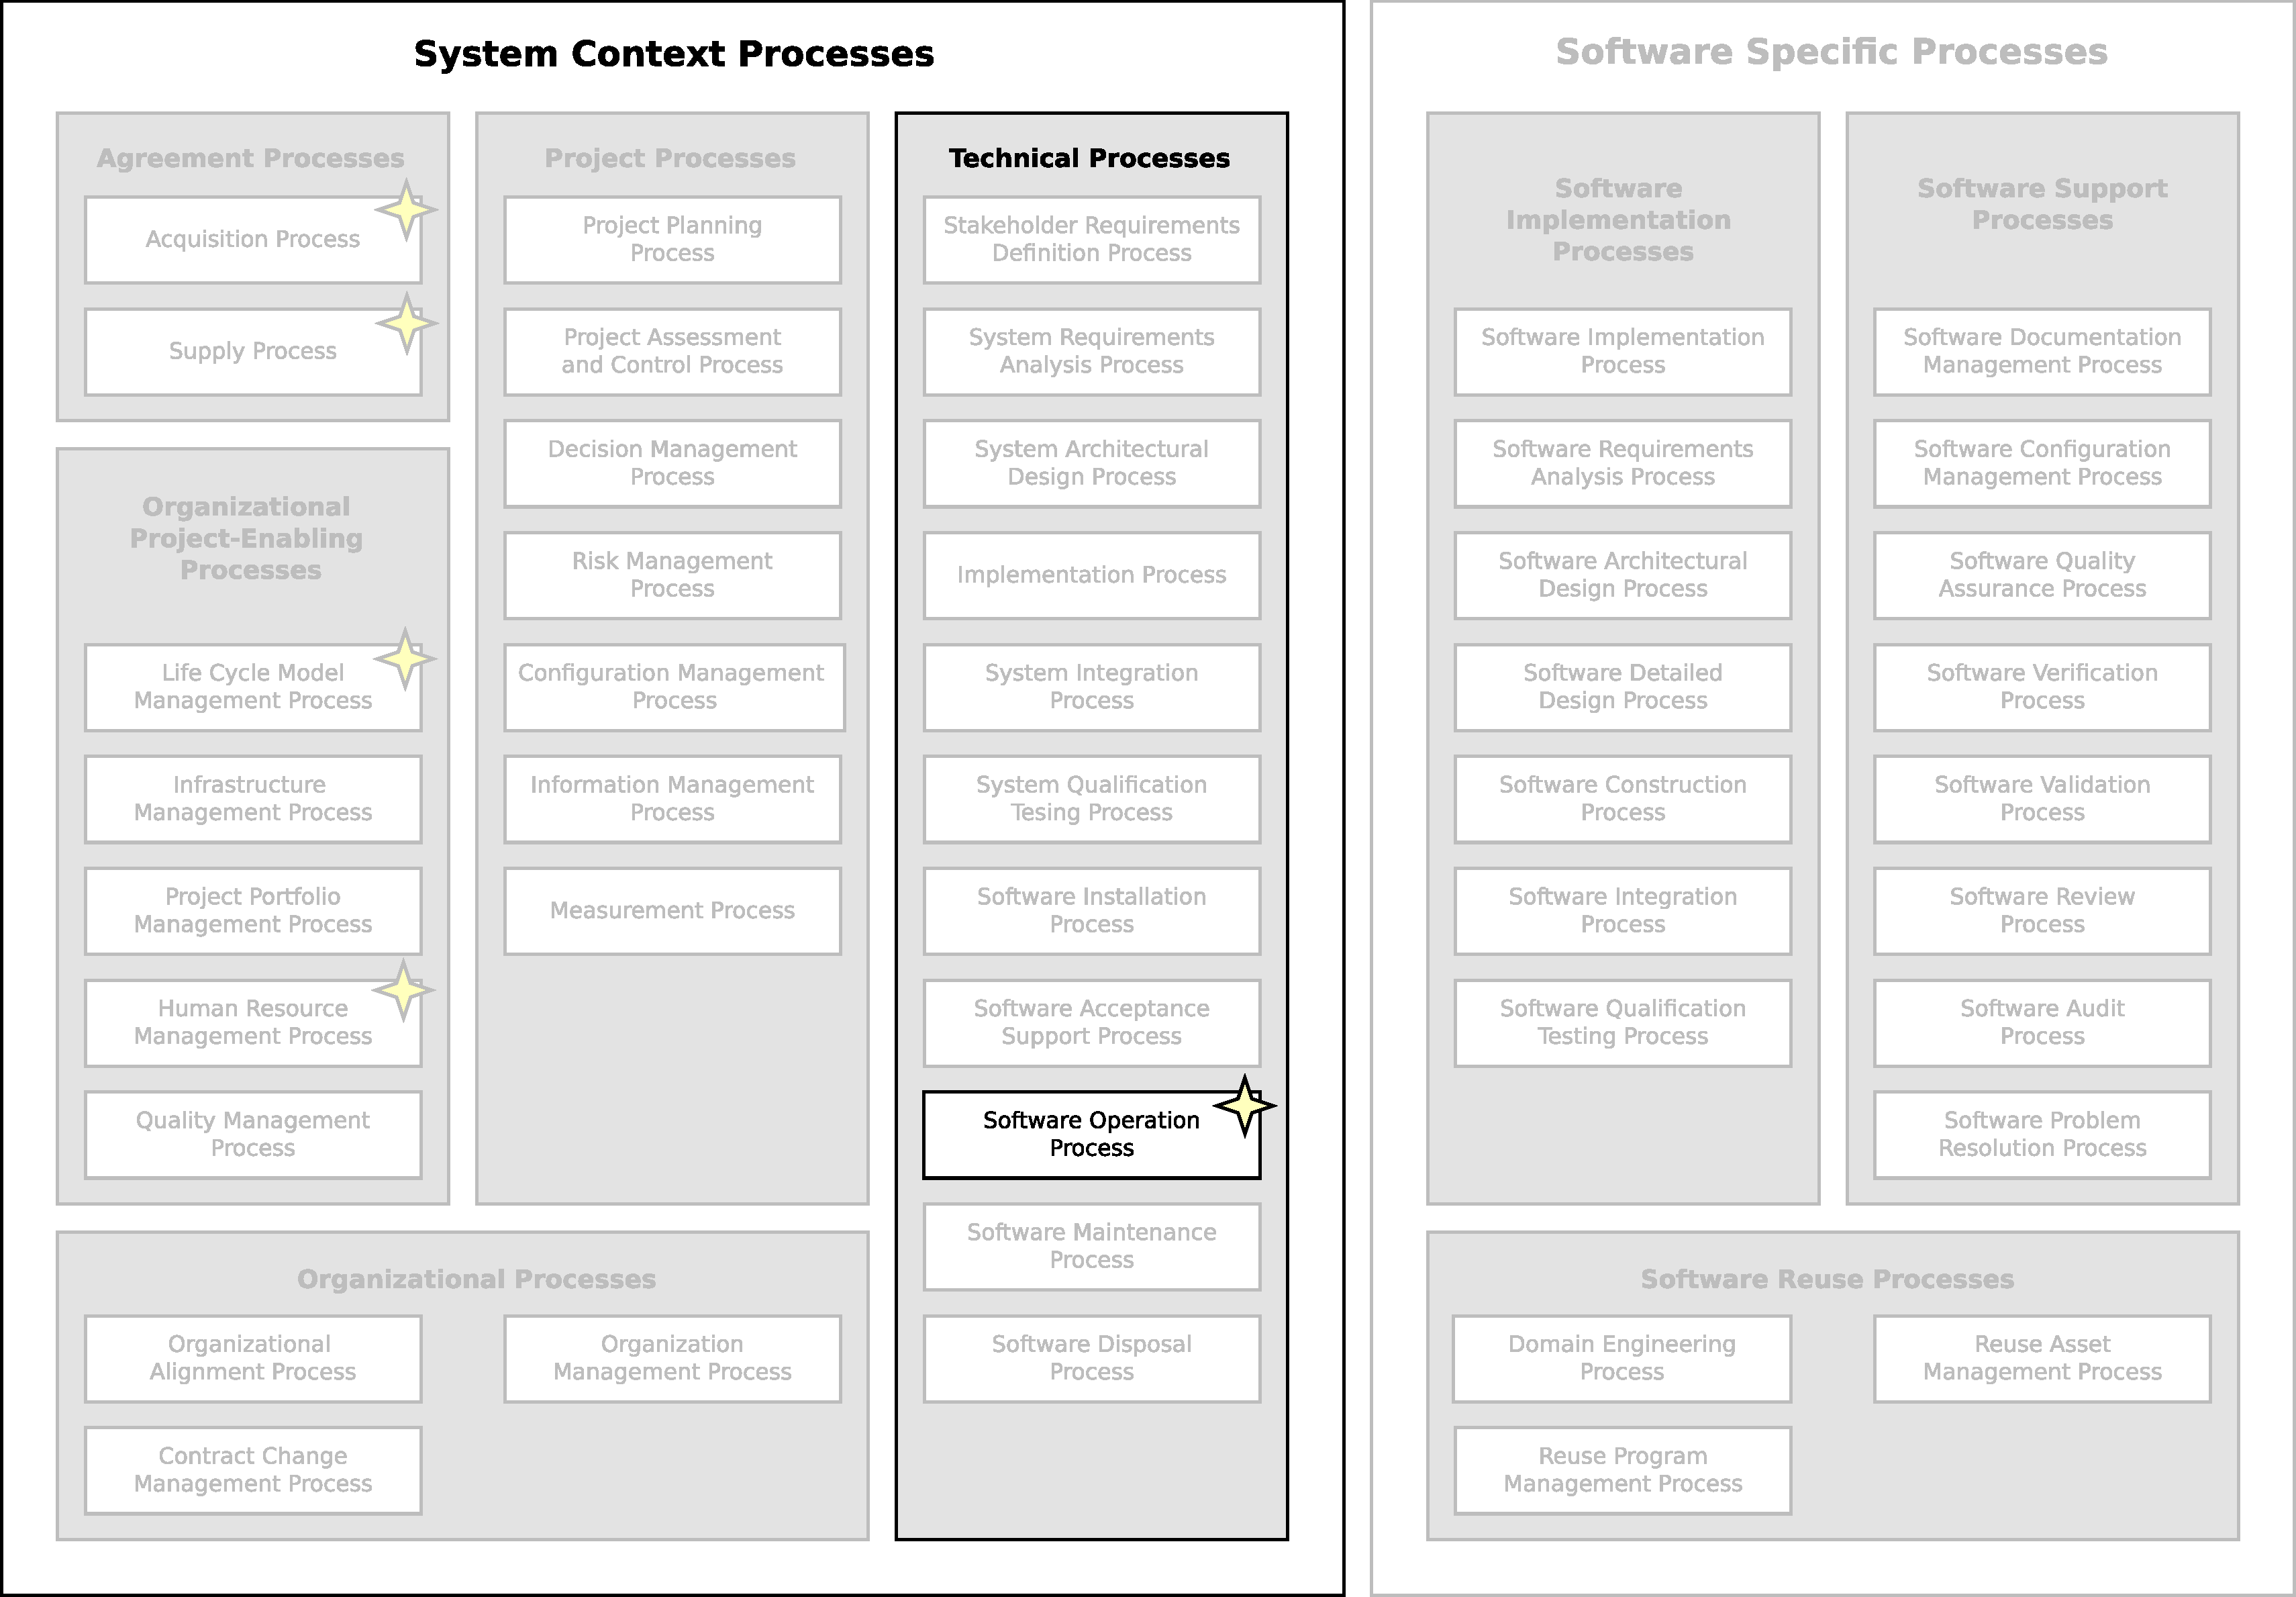
\includegraphics[width=15cm,keepaspectratio]{figures/life-cycle-process-groups-lower-level-software-operation-processes.pdf}
		\caption{Software Operation Process Lower-Level Processes}
		\label{fig:lower_level_software_operation_processes}
	\end{figure}

		\subsubsection{OPERATIONAL USE PROCESS\label{llproc:operational_use_process}}

			\subsubsubsection{PURPOSE}
			\begin{adjustwidth}{2em}{0pt} 

				The purpose of the \nameref{llproc:operational_use_process} is to ensure the correct and efficient operation of the product for the duration of its intended usage and in its installed environment.

				This process is a lower-level process of the \nameref{proc:software_operation_process}. It replaces the Operational Use activity.

			\end{adjustwidth}

			\subsubsubsection{OUTCOMES}
			\begin{adjustwidth}{2em}{0pt} 

				\begin{compactitem}

					\item operational risks for the product introduction and operation are identified and monitored;

					\item the product is operated in its intended environment according to requirements; and

					\item criteria for the operational use are developed that demonstrates compliance with the agreed requirements.

				\end{compactitem}

			\end{adjustwidth}

		\subsubsection{CUSTOMER SUPPORT PROCESS\label{llproc:customer_support_process}}

			\subsubsubsection{PURPOSE}
			\begin{adjustwidth}{2em}{0pt} 

				The purpose of the \nameref{llproc:customer_support_process} is to establish and maintain an acceptable level of service through assistance and consultation to the customer to support effective use of the product.

				This process is a lower-level process of the \nameref{proc:software_operation_process}. It replaces the Customer Support activity.

			\end{adjustwidth}

			\subsubsubsection{OUTCOMES}
			\begin{adjustwidth}{2em}{0pt} 

				\begin{compactitem}

					\item service needs for customer support are identified and monitored on an ongoing basis;

					\item customer satisfaction with both the support services being provided and the product itself is evaluated on an ongoing basis;

					\item operational support is provided by handling customer inquiries and requests and resolving operational problems; and

					\item customer support needs are met through delivery of appropriate services.

				\end{compactitem}

			\end{adjustwidth}
